\documentclass[11pt,compsoc]{IEEEtran}
\usepackage[spanish]{babel}
\usepackage{amsmath,amsfonts}
\usepackage{algorithmic}
\usepackage{array}
\usepackage[caption=false,font=normalsize,labelfont=sf,textfont=sf]{subfig}
\usepackage{textcomp}
\usepackage{stfloats}
\usepackage{url}
\usepackage{verbatim}
\usepackage{graphicx}
\hyphenation{op-tical net-works semi-conduc-tor IEEE-Xplore}
\def\BibTeX{{\rm B\kern-.05em{\sc i\kern-.025em b}\kern-.08em
		T\kern-.1667em\lower.7ex\hbox{E}\kern-.125emX}}
\usepackage{balance}
\begin{document}
	\title{El procesador CELL, desde un enfoque
		histórico}
	\author{Ramiro Barcala Roca, Valentin Angrigiani, Gabriel Hackl}
		
	\markboth{Organizacion del Computador, Catedra Marchi, 2024}%
	{How to Use the IEEEtran \LaTeX \ Templates}
	\maketitle
	
	\begin{abstract}
		Este trabajo tratará el procesador CELL de Sony. Se toma un enfoque investigativo y contrastante entre arquitecturas del CELL, y otras de la época (y la actualidad). Las aplicaciones principales para las que fue diseñado, y las aplicaciones que se descubrieron luego junto  con su importancia histórica. Conceptos básicos de computación heterogénea (distintos nucleos). Analisis a futuro relacionandolo a todo.
	\end{abstract}
	
	\begin{IEEEkeywords}
		SPE,PPE,SIMD,.
	\end{IEEEkeywords}
	
	\section{Introducción}
	\IEEEPARstart{A} mediados de los 2000, la empresa Sony empieza a investigar y desarrollar su sistema de entretenimiento "Play-Station 3". Todo esto en un mercado competitivo frente a otras marcas como Microsoft y Nintendo. Terminan con un procesador multi-core, el cual tiene como particularidades los sub-nucleos. Sony tambien quería estandarizar su procesador en dispositivos de todas las gamas y usos multimedias.
	
	Sin embargo, tanto el producto como su procesador,fueron un fracaso comercial. Sin embargo, se descubriero usos investigativos/científicos/economicos, entre otros.
	
	
	\section{Epoca Pre-CELL}
	\noindent Para ponernos en contexto, vamos a explicar la situacion de las arquitecturas del momento, como de las empresas que lanzaban nuevos productos (del mismo rubro o parecido), en aquella época.
	
	\subsection{Empresas del rubro de las consolas}
	\noindent 
	En el año 2005, las siguientes empresas de consolas/videojuegos, competian en el mercado: 
		\begin{itemize}
		\item{{\bf{Sony}}: parte de un exito rotundo con su anterior producto: la PS2. Tenia grandes expectativas con su nuevo producto, apuesta a lo grande, con nuevas funcionalidades no esenciales (ej: puertos HDMI, Blue-Ray, etc).}
		
		\item{{\bf{Microsoft}}: viene de un exito modesto, con su primer producto: la X-Box. En la X-Box 360, se centra en abaratar su producto, pero proveer servicios en linea de gran calidad. Esto les pasa factura con los problemas de hardware que tendria la consola mas adelante.}
		
		\item{{\bf{Nintendo}}: tuvo un exito pobre en su consola anterior, la Gamecube. En la Wii, se decide no hacer costos de fabricacion muy caros. Pero además, se centra en facilitar experiencias novedosas para el usuario final, mediante el uso de movimientos corporales para controlar los juegos, como extensiones al mismo control (volantes, soportes, etc).}
		\end{itemize}
		
	Para comprender un poco mas la magnitud del la importancia del mercado, los siguiente graficos muestran como alrededor de esos años, la industria de los videojuegos crece de una manera formidable, tanto como la porcion del mercado de cada empresa.\\
	
	\begin{center}
		{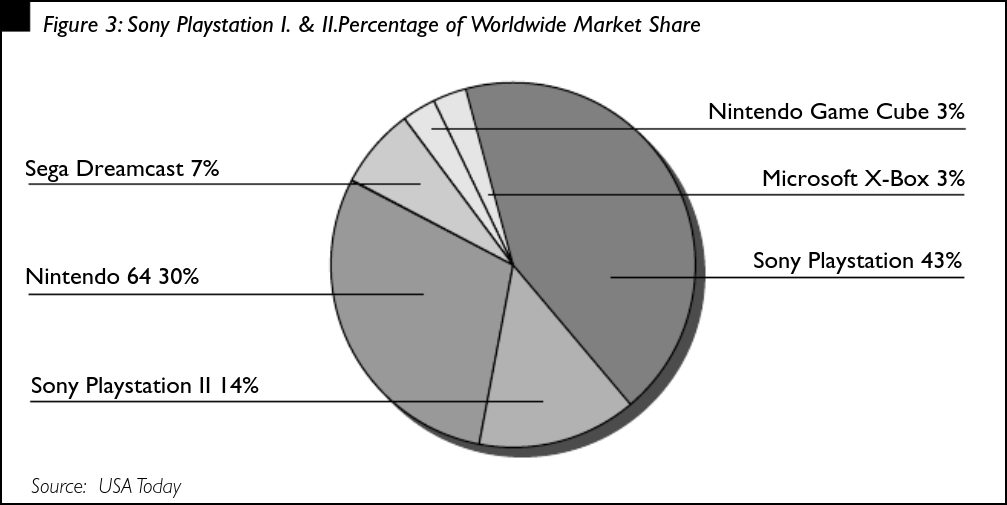
\includegraphics[width=3in,height=2in,clip,keepaspectratio]{imgs/marketshare.png}}\newline
		
		
		{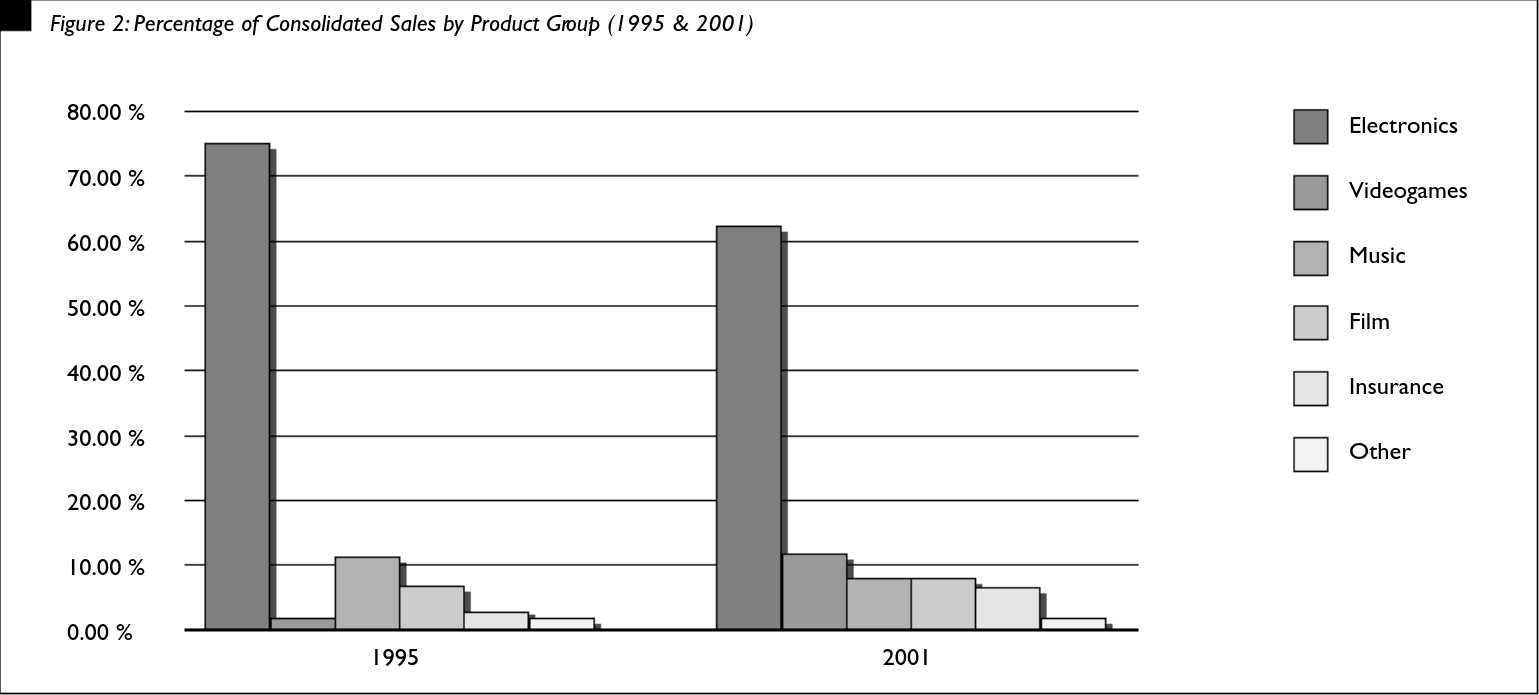
\includegraphics[width=3in,height=2in,clip,keepaspectratio]{imgs/gamingshare.png}}\newline
	\end{center}
	
	
	\section{Arquitectura CELL}	% MODULOS,ARQUITECTURAS INTERNAS, CONVENCIONES, INSTRUCCIONES, etc
	\noindent Diseñada por Sony, en conjunto con Toshiba e IBM, esta arquitectura trae al mercado un procesador que maneja fuertemente la computacion heterogenea, mediante el uso de sus 9 nucleos.  
	
	\subsection{Modulos, en general y separado} 
	\noindent 
	
	\subsection{Interconexion} 
	\noindent 
	
	\subsection{Computacion heterogenea }
	\noindent 
	
	\subsection{Computacion heterogenea en el Cell }% SIMD
	\noindent 
	
	\subsection{Diferencias con arquitecturas actuales}% SIMD
	\noindent 
	
	\subsection{Arquitecturas de la competencia}%ARQUITECTURAS DEL MOMENTO
	
	
	
	\section{Inconveniencias}
	\noindent Debido a que programar los distintos SSP requerían mucho tiempo, una gran cantidad  de desarrolladores pasaron por alto los programas apartes que requerian los mismos, y se centraban unicamente en el PPE. De modo que, todas las tareas eran realizadas por el PPE, lo cual provocó bajos rendimientos en los programas que corria el CELL, ya que sus SPE's quedaban inutilizados.
	
	Muchas tareas que se podian paralelizar, no se estaban ejecutando como debían, ni por los sub-nucleos especializados para eso. 
	
	Esto 
		
	
	
	\section{Aplicaciones del CELL}
	\noindent
	
	\subsection{Puntos fuerte}
	\noindent
	
	\subsection{Research and Development}
	\noindent
	
	
	
	\section{Remanentes del Cell en la Actualidad}%Importancia historica
	\noindent 
	
	
	
	
	
	
	
	\section{Analisis a futuro}
	\noindent 
	
	
	
	
	
	
	\section{Conclusion}
	\noindent
	
	
		\begin{thebibliography}{1}
			
			\bibitem{ams}
			{\it{Laboratorio de Arquitecturas Avanzadas con Cell y PlayStation 3}}, Universitat de València, por Fernando Pardo y Jose A. Boluda.
			
			\bibitem{oxford}
			{\it{Un vistazo al pasado, ¿cómo de potente fue PS3? }},https://www.3djuegos.com/ps3/noticias/un-vistazo-al-pasado-como-de-potente-fue-ps3-190331-91210
		
			\bibitem{ams}
			{\it{The PlayStation Supercomputer}}, https://www.datacenterdynamics.com/en/analysis/the-playstation-supercomputer/
			
			\bibitem{ams}
			{\it{The Untold Story of the Cell Processor: Sony's Pioneering Technology in Gaming}}, https://www.gameversedaily.com/post/the-untold-story-of-the-cell-processor-sony-s-pioneering-technology-in-gaming
			
			\bibitem{ams}
			{\it{Console wars: A rare bright spot in the gloomy technology industry, video games are growing up}}, 
			https://www.economist.com/business/2002/06/20/console-wars
			
			\bibitem{ams}
			{\it{Console wars}}, 			https://www.ft.com/content/ef24f36e-5c54-11dc-9cc9-0000779fd2ac
			
			\bibitem{ams}
			{\it{Console wars}}, 			
			https://www.gainesville.com/story/news/2006/11/11/waging-console-war/31502430007/
			
			\bibitem{ams}
			{\it{PlayStation 3, Console Wars and the Costs of Complexity}}, 			
			https://techliberation.com/2006/09/07/playstation-3-console-wars-the-costs-of-complexity/
			
			\bibitem{ams}
			{\it{Console giants square up}}, 			
			http://news.bbc.co.uk/2/hi/entertainment/2002112.stm
			
			\bibitem{ams}
			{\it{Report from the video game wars: Wii vs. PS3 vs. Xbox360}}, 
			https://fabricegrinda.com/report-from-the-video-game-wars-wii-vs-ps3-vs-xbox360/
			
			\bibitem{ams}
			{\it{Report from the video game wars: Wii vs. PS3 vs. Xbox360}}, 
			https://www.copetti.org/writings/consoles/
		
		\end{thebibliography}
		
			
	
		
\end{document}
